\RequirePackage{luatex85}
\documentclass[tikz]{standalone}
% Default preamble
\usepackage{pgfplots}
\pgfplotsset{compat=newest}
\usepgfplotslibrary{groupplots}
\usepgfplotslibrary{polar}
\usepgfplotslibrary{smithchart}
\usepgfplotslibrary{statistics}
\usepgfplotslibrary{dateplot}
\usepgfplotslibrary{ternary}
\begin{document}
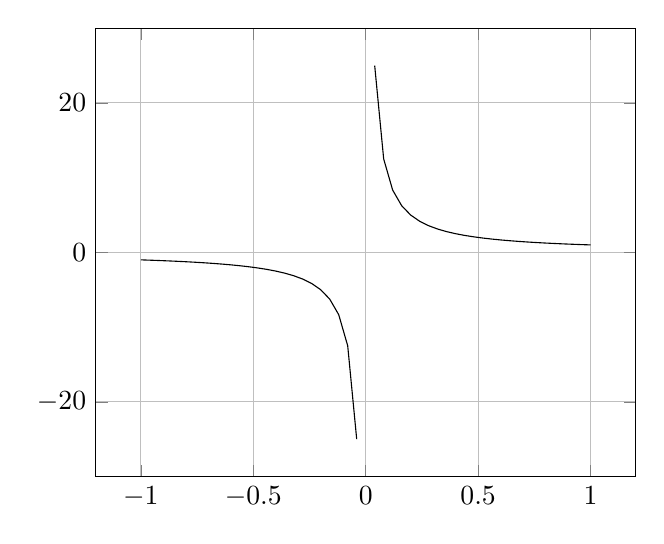
\begin{tikzpicture}
\begin{axis}[xmajorgrids, ymajorgrids]
    \addplot[no marks]
        coordinates {
            (-1.0,-1.0)
            (-0.96,-1.0416666666666667)
            (-0.92,-1.0869565217391304)
            (-0.88,-1.1363636363636365)
            (-0.84,-1.1904761904761905)
            (-0.8,-1.25)
            (-0.76,-1.3157894736842106)
            (-0.72,-1.3888888888888888)
            (-0.68,-1.4705882352941175)
            (-0.64,-1.5625)
            (-0.6,-1.6666666666666667)
            (-0.56,-1.7857142857142856)
            (-0.52,-1.923076923076923)
            (-0.48,-2.0833333333333335)
            (-0.44,-2.272727272727273)
            (-0.4,-2.5)
            (-0.36,-2.7777777777777777)
            (-0.32,-3.125)
            (-0.28,-3.571428571428571)
            (-0.24,-4.166666666666667)
            (-0.2,-5.0)
            (-0.16,-6.25)
            (-0.12,-8.333333333333334)
            (-0.08,-12.5)
            (-0.04,-25.0)

            (0.04,25.0)
            (0.08,12.5)
            (0.12,8.333333333333334)
            (0.16,6.25)
            (0.2,5.0)
            (0.24,4.166666666666667)
            (0.28,3.571428571428571)
            (0.32,3.125)
            (0.36,2.7777777777777777)
            (0.4,2.5)
            (0.44,2.272727272727273)
            (0.48,2.0833333333333335)
            (0.52,1.923076923076923)
            (0.56,1.7857142857142856)
            (0.6,1.6666666666666667)
            (0.64,1.5625)
            (0.68,1.4705882352941175)
            (0.72,1.3888888888888888)
            (0.76,1.3157894736842106)
            (0.8,1.25)
            (0.84,1.1904761904761905)
            (0.88,1.1363636363636365)
            (0.92,1.0869565217391304)
            (0.96,1.0416666666666667)
            (1.0,1.0)
        }
        ;
\end{axis}
\end{tikzpicture}
\end{document}
